\documentclass[]{book}
\usepackage{lmodern}
\usepackage{amssymb,amsmath}
\usepackage{ifxetex,ifluatex}
\usepackage{fixltx2e} % provides \textsubscript
\ifnum 0\ifxetex 1\fi\ifluatex 1\fi=0 % if pdftex
  \usepackage[T1]{fontenc}
  \usepackage[utf8]{inputenc}
\else % if luatex or xelatex
  \ifxetex
    \usepackage{mathspec}
  \else
    \usepackage{fontspec}
  \fi
  \defaultfontfeatures{Ligatures=TeX,Scale=MatchLowercase}
\fi
% use upquote if available, for straight quotes in verbatim environments
\IfFileExists{upquote.sty}{\usepackage{upquote}}{}
% use microtype if available
\IfFileExists{microtype.sty}{%
\usepackage{microtype}
\UseMicrotypeSet[protrusion]{basicmath} % disable protrusion for tt fonts
}{}
\usepackage[margin=1in]{geometry}
\usepackage{hyperref}
\hypersetup{unicode=true,
            pdftitle={Examining Work With Data in STEM Education Through the Lens of Engagement Theory: A Person-Oriented Approach Using an Experience Sampling Method},
            pdfauthor={Joshua M. Rosenberg},
            pdfborder={0 0 0},
            breaklinks=true}
\urlstyle{same}  % don't use monospace font for urls
\usepackage{natbib}
\bibliographystyle{apalike}
\usepackage{color}
\usepackage{fancyvrb}
\newcommand{\VerbBar}{|}
\newcommand{\VERB}{\Verb[commandchars=\\\{\}]}
\DefineVerbatimEnvironment{Highlighting}{Verbatim}{commandchars=\\\{\}}
% Add ',fontsize=\small' for more characters per line
\usepackage{framed}
\definecolor{shadecolor}{RGB}{248,248,248}
\newenvironment{Shaded}{\begin{snugshade}}{\end{snugshade}}
\newcommand{\KeywordTok}[1]{\textcolor[rgb]{0.13,0.29,0.53}{\textbf{#1}}}
\newcommand{\DataTypeTok}[1]{\textcolor[rgb]{0.13,0.29,0.53}{#1}}
\newcommand{\DecValTok}[1]{\textcolor[rgb]{0.00,0.00,0.81}{#1}}
\newcommand{\BaseNTok}[1]{\textcolor[rgb]{0.00,0.00,0.81}{#1}}
\newcommand{\FloatTok}[1]{\textcolor[rgb]{0.00,0.00,0.81}{#1}}
\newcommand{\ConstantTok}[1]{\textcolor[rgb]{0.00,0.00,0.00}{#1}}
\newcommand{\CharTok}[1]{\textcolor[rgb]{0.31,0.60,0.02}{#1}}
\newcommand{\SpecialCharTok}[1]{\textcolor[rgb]{0.00,0.00,0.00}{#1}}
\newcommand{\StringTok}[1]{\textcolor[rgb]{0.31,0.60,0.02}{#1}}
\newcommand{\VerbatimStringTok}[1]{\textcolor[rgb]{0.31,0.60,0.02}{#1}}
\newcommand{\SpecialStringTok}[1]{\textcolor[rgb]{0.31,0.60,0.02}{#1}}
\newcommand{\ImportTok}[1]{#1}
\newcommand{\CommentTok}[1]{\textcolor[rgb]{0.56,0.35,0.01}{\textit{#1}}}
\newcommand{\DocumentationTok}[1]{\textcolor[rgb]{0.56,0.35,0.01}{\textbf{\textit{#1}}}}
\newcommand{\AnnotationTok}[1]{\textcolor[rgb]{0.56,0.35,0.01}{\textbf{\textit{#1}}}}
\newcommand{\CommentVarTok}[1]{\textcolor[rgb]{0.56,0.35,0.01}{\textbf{\textit{#1}}}}
\newcommand{\OtherTok}[1]{\textcolor[rgb]{0.56,0.35,0.01}{#1}}
\newcommand{\FunctionTok}[1]{\textcolor[rgb]{0.00,0.00,0.00}{#1}}
\newcommand{\VariableTok}[1]{\textcolor[rgb]{0.00,0.00,0.00}{#1}}
\newcommand{\ControlFlowTok}[1]{\textcolor[rgb]{0.13,0.29,0.53}{\textbf{#1}}}
\newcommand{\OperatorTok}[1]{\textcolor[rgb]{0.81,0.36,0.00}{\textbf{#1}}}
\newcommand{\BuiltInTok}[1]{#1}
\newcommand{\ExtensionTok}[1]{#1}
\newcommand{\PreprocessorTok}[1]{\textcolor[rgb]{0.56,0.35,0.01}{\textit{#1}}}
\newcommand{\AttributeTok}[1]{\textcolor[rgb]{0.77,0.63,0.00}{#1}}
\newcommand{\RegionMarkerTok}[1]{#1}
\newcommand{\InformationTok}[1]{\textcolor[rgb]{0.56,0.35,0.01}{\textbf{\textit{#1}}}}
\newcommand{\WarningTok}[1]{\textcolor[rgb]{0.56,0.35,0.01}{\textbf{\textit{#1}}}}
\newcommand{\AlertTok}[1]{\textcolor[rgb]{0.94,0.16,0.16}{#1}}
\newcommand{\ErrorTok}[1]{\textcolor[rgb]{0.64,0.00,0.00}{\textbf{#1}}}
\newcommand{\NormalTok}[1]{#1}
\usepackage{longtable,booktabs}
\usepackage{graphicx,grffile}
\makeatletter
\def\maxwidth{\ifdim\Gin@nat@width>\linewidth\linewidth\else\Gin@nat@width\fi}
\def\maxheight{\ifdim\Gin@nat@height>\textheight\textheight\else\Gin@nat@height\fi}
\makeatother
% Scale images if necessary, so that they will not overflow the page
% margins by default, and it is still possible to overwrite the defaults
% using explicit options in \includegraphics[width, height, ...]{}
\setkeys{Gin}{width=\maxwidth,height=\maxheight,keepaspectratio}
\IfFileExists{parskip.sty}{%
\usepackage{parskip}
}{% else
\setlength{\parindent}{0pt}
\setlength{\parskip}{6pt plus 2pt minus 1pt}
}
\setlength{\emergencystretch}{3em}  % prevent overfull lines
\providecommand{\tightlist}{%
  \setlength{\itemsep}{0pt}\setlength{\parskip}{0pt}}
\setcounter{secnumdepth}{5}
% Redefines (sub)paragraphs to behave more like sections
\ifx\paragraph\undefined\else
\let\oldparagraph\paragraph
\renewcommand{\paragraph}[1]{\oldparagraph{#1}\mbox{}}
\fi
\ifx\subparagraph\undefined\else
\let\oldsubparagraph\subparagraph
\renewcommand{\subparagraph}[1]{\oldsubparagraph{#1}\mbox{}}
\fi

%%% Use protect on footnotes to avoid problems with footnotes in titles
\let\rmarkdownfootnote\footnote%
\def\footnote{\protect\rmarkdownfootnote}

%%% Change title format to be more compact
\usepackage{titling}

% Create subtitle command for use in maketitle
\newcommand{\subtitle}[1]{
  \posttitle{
    \begin{center}\large#1\end{center}
    }
}

\setlength{\droptitle}{-2em}
  \title{Examining Work With Data in STEM Education Through the Lens of
Engagement Theory: A Person-Oriented Approach Using an Experience
Sampling Method}
  \pretitle{\vspace{\droptitle}\centering\huge}
  \posttitle{\par}
  \author{Joshua M. Rosenberg}
  \preauthor{\centering\large\emph}
  \postauthor{\par}
  \predate{\centering\large\emph}
  \postdate{\par}
  \date{2018-02-23}

\usepackage{booktabs}

\begin{document}
\maketitle

{
\setcounter{tocdepth}{1}
\tableofcontents
}
\chapter{Abstract}\label{abstract}

This study will examine how 203 early adolescent learners work with
data, or engage in activities focused on constructing measures of and
modeling data, in the context of STEM summer enrichment programs. Video
recordings of programs will be coded to identify the presence of five
aspects of learners' work with data: asking questions or identifying
problems, constructing measures, collecting data, accounting for
variability or uncertainty, and interpreting and communicating findings.
Additionally, measures of instructional support for such practices will
be used, so codes for work with data with instructional support are also
created. Youth's responses to the Experience Sampling Method (ESM) will
be used to examine their cognitive, behavioral, and affective engagement
as well as their perceptions of challenge and competence. A
person-oriented analytic approach will be used to identify profiles of
engagement that will help us to understand how learners engage in work
with data. Examining work with data in terms of contemporary engagement
theory can help us to understand these key STEM activities in terms of
learner's experience, which past research suggests impacts student
learning, yet which has not been brought to bear on the topic of work
with data. Knowing more about students' engagement can help us to design
activities and interventions around work with data that are highly
engaging to students and that support their capabilities to work with
data.

\chapter{Introduction}\label{intro-placemarker}

Changes in how we plan our day-to-day lives, communicate, and learn are
increasingly impacted by data. These sources of data are created by us,
for us, and about us, although at present opportunities for learners to
analyze data in educational settings remain limited. Data analysis
includes processes of collecting, creating, modeling data, and asking
questions that may be answered with data and making sense of findings.
Analyzing data in educational settings, then, is more than just
crunching numbers or interpreting a figure created by someone else, but
rather is about making sense of phenomena and problem solving (Wild \&
Pfannkuch, 1999). Data analysis and its processes cut across STEM
domains and are recognized as core competencies in both the Next
Generation Science Standards and the Common Core State Standards
(National Governors Association Center for Best Practices, Council of
Chief State School Officers, 2010; NGSS Lead States, 2013). Scholars
have pointed out the benefits of analyzing data for learners as young as
two years old (Gopnik, \& Sobel, 2000).

In supporting teachers and learners' data analysis efforts, some
scholars have focused on the process of key data analytic practices,
particularly the practices of generating measures of phenomena and
creating data models---as an organizing activity in science and
mathematics content areas (English, 2012; Lehrer \& Romberg, 1996; Lesh,
Middleton, Caylor, \& Gupta, 2008). Findings from this area of research
suggest that engaging in these practices ``has an exceptionally high
payoff in terms of students' scientific reasoning'' (Lehrer \& Schauble,
2015, p.~696) and can highlight the utility of mathematics for students'
lives (Lesh, Middleton, Caylor, \& Gupta, 2008).

While scholars have looked at cognitive outcomes and learners'
capability to participate in specific, key aspects of data analysis as
well as strategies to address key challenges of doing so, we have not
yet examined key data analytic practices in terms of engagement theory.
Contemporary engagement theory offers a framework with which to
understand learners' experience of engaging in these practices, referred
to as work with data in the remainder of this study because it considers
multiple dimensions of experiencing engagement and its dynamic nature
(Fredricks \& McColskey, 2012). Scholars commonly consider engagement in
terms of its cognitive (i.e., use of meta-cognitive learning
strategies), behavioral (hard work on a task), and affective dimensions
(enjoyment; Fredricks, Blumenfeld, \& Paris, 2004; Sinatra, Heddy, \&
Lombardi, 2015; Skinner \& Pitzer, 2012).

In recognition of its dynamic nature, some engagement scholars have
usefully drawn upon flow theory (Csikszentmihalyi, 1990, 1997) to
identify how learners' perceived competence and challenge act as key
conditions of engagement (Shernoff, Kelly, Tonks, Anderson, Cavanagh,
Sinha, \& Abdi, 2016), aligning with situated views of learning (Sfard,
1998) and motivation (Nolen, Horn, \& Ward, 2015).

The purpose of this study, then, is to understand learners' experience
of engagement in work with data and the conditions that support it.
Engagement is understood in terms of cognitive, behavioral, and
affective dimensions, and the conditions that support engagement are
understood in terms of two subjective components that past research and
theory suggest influence engagement: perceived challenge and perceived
competence, as well as instructional support for engaging in aspects of
work with data. Engagement in work with data is explored in the context
of outside-of-school STEM enrichment programs carried out during the
summer. In recognition of the challenge of studying engagement in
learning environments where factors related to activities, learners, and
each of the nine programs all interact at the same time, this study uses
a methodological approach suited to studying engagement as a dynamic,
multi-faceted experience. Specifically, this study employs the
Experience Sampling Method (ESM; Hektner, Schmidt, \& Csikszentmihalyi,
2007) where learners answer short questions about their experience when
signaled. This approach is both sensitive to changes in engagement over
time, as well as between learners and allows us to understand engagement
and how factors impact it in more nuanced and complex ways (Turner \&
Meyer, 2000).

\chapter{Literature Review}\label{literature-review}

Placeholder

\section{Defining Work With Data}\label{defining-work-with-data}

\section{What We Know (And Do Not Know) About Engagement in Work with
Data}\label{what-we-know-and-do-not-know-about-engagement-in-work-with-data}

\section{Engagement in STEM Domains}\label{engagement-in-stem-domains}

\section{Using ESM to Study the Dynamics of
Engagement}\label{using-esm-to-study-the-dynamics-of-engagement}

\section{A Person-Oriented Approach to
Engagement}\label{a-person-oriented-approach-to-engagement}

\section{Need for the Present Study}\label{need-for-the-present-study}

\section{Conceptual Framework}\label{conceptual-framework}

\section{Research Questions}\label{research-questions}

\chapter{Method}\label{method}

Placeholder

\section{Participants}\label{participants}

\section{Context}\label{context}

\section{Procedure}\label{procedure}

\section{Data Sources and Measures}\label{data-sources-and-measures}

\section{Data Analysis}\label{data-analysis}

\section{Power Analysis}\label{power-analysis}

\section{Limitations}\label{limitations}

\chapter{Results}\label{results}

In this section, results in terms of \ldots{}

\begin{Shaded}
\begin{Highlighting}[]
\NormalTok{esm <-}\StringTok{ }\KeywordTok{read_csv}\NormalTok{(}\StringTok{"/Volumes/SCHMIDTLAB/PSE/data/STEM-IE/STEM-IE-esm.csv"}\NormalTok{)}
\NormalTok{pre_survey_data_processed <-}\StringTok{ }\KeywordTok{read_csv}\NormalTok{(}\StringTok{"/Volumes/SCHMIDTLAB/PSE/data/STEM-IE/STEM-IE-pre-survey.csv"}\NormalTok{)}
\NormalTok{post_survey_data_partially_processed <-}\StringTok{ }\KeywordTok{read_csv}\NormalTok{(}\StringTok{"/Volumes/SCHMIDTLAB/PSE/data/STEM-IE/STEM-IE-post-survey.csv"}\NormalTok{)}
\NormalTok{video <-}\StringTok{ }\KeywordTok{read_csv}\NormalTok{(}\StringTok{"/Volumes/SCHMIDTLAB/PSE/data/STEM-IE/STEM-IE-video.csv"}\NormalTok{)}
\NormalTok{pqa <-}\StringTok{ }\KeywordTok{read_csv}\NormalTok{(}\StringTok{"/Volumes/SCHMIDTLAB/PSE/data/STEM-IE/STEM-IE-pqa.csv"}\NormalTok{)}
\NormalTok{attendance <-}\StringTok{ }\KeywordTok{read_csv}\NormalTok{(}\StringTok{"/Volumes/SCHMIDTLAB/PSE/data/STEM-IE/STEM-IE-attendance.csv"}\NormalTok{)}
\NormalTok{class_data <-}\StringTok{ }\KeywordTok{read_csv}\NormalTok{(}\StringTok{"/Volumes/SCHMIDTLAB/PSE/data/STEM-IE/STEM-IE-class-video.csv"}\NormalTok{)}
\NormalTok{demographics <-}\StringTok{ }\KeywordTok{read_csv}\NormalTok{(}\StringTok{"/Volumes/SCHMIDTLAB/PSE/data/STEM-IE/STEM-IE-demographics.csv"}\NormalTok{)}
\NormalTok{pm <-}\StringTok{ }\KeywordTok{read_csv}\NormalTok{(}\StringTok{"/Volumes/SCHMIDTLAB/PSE/Data/STEM-IE/STEM-IE-program-match.csv"}\NormalTok{)}
\end{Highlighting}
\end{Shaded}

\begin{Shaded}
\begin{Highlighting}[]
\CommentTok{# save.image("~/desktop/sandbox-01.Rdata")}
\KeywordTok{load}\NormalTok{(}\StringTok{"~/desktop/sandbox-01.Rdata"}\NormalTok{)}
\end{Highlighting}
\end{Shaded}

\begin{Shaded}
\begin{Highlighting}[]
\NormalTok{attendance <-}\StringTok{ }\KeywordTok{rename}\NormalTok{(attendance, }\DataTypeTok{participant_ID =}\NormalTok{ ParticipantID)}
\NormalTok{attendance <-}\StringTok{ }\KeywordTok{mutate}\NormalTok{(attendance, }\DataTypeTok{prop_attend =}\NormalTok{ DaysAttended }\OperatorTok{/}\StringTok{ }\NormalTok{DaysScheduled, }
                     \DataTypeTok{participant_ID =} \KeywordTok{as.integer}\NormalTok{(participant_ID))}
\NormalTok{attendance <-}\StringTok{ }\KeywordTok{select}\NormalTok{(attendance, participant_ID, prop_attend)}

\NormalTok{demographics <-}\StringTok{ }\KeywordTok{filter}\NormalTok{(demographics, participant_ID}\OperatorTok{!=}\StringTok{ }\DecValTok{7187}\NormalTok{)}
\NormalTok{demographics <-}\StringTok{ }\KeywordTok{left_join}\NormalTok{(demographics, attendance)}

\NormalTok{esm}\OperatorTok{$}\NormalTok{overall_engagement <-}\StringTok{ }\NormalTok{jmRtools}\OperatorTok{::}\KeywordTok{composite_mean_maker}\NormalTok{(esm, hard_working, concentrating, enjoy, interest)}
\end{Highlighting}
\end{Shaded}

\begin{Shaded}
\begin{Highlighting}[]
\NormalTok{df <-}\StringTok{ }\KeywordTok{left_join}\NormalTok{(esm, pre_survey_data_processed, }\DataTypeTok{by =} \StringTok{"participant_ID"}\NormalTok{) }\CommentTok{# df & post-survey}
\NormalTok{df <-}\StringTok{ }\KeywordTok{left_join}\NormalTok{(df, video, }\DataTypeTok{by =} \KeywordTok{c}\NormalTok{(}\StringTok{"program_ID"}\NormalTok{, }\StringTok{"response_date"}\NormalTok{, }\StringTok{"sociedad_class"}\NormalTok{, }\StringTok{"signal_number"}\NormalTok{)) }\CommentTok{# df & video}
\NormalTok{df <-}\StringTok{ }\KeywordTok{left_join}\NormalTok{(df, demographics, }\DataTypeTok{by =} \KeywordTok{c}\NormalTok{(}\StringTok{"participant_ID"}\NormalTok{, }\StringTok{"program_ID"}\NormalTok{)) }\CommentTok{# df and demographics}
\end{Highlighting}
\end{Shaded}

\begin{Shaded}
\begin{Highlighting}[]
\NormalTok{pqa <-}\StringTok{ }\KeywordTok{mutate}\NormalTok{(pqa, }
              \DataTypeTok{active =}\NormalTok{ active_part_}\DecValTok{1} \OperatorTok{+}\StringTok{ }\NormalTok{active_part_}\DecValTok{2}\NormalTok{,}
              \DataTypeTok{ho_thinking =}\NormalTok{ ho_thinking_}\DecValTok{1} \OperatorTok{+}\StringTok{ }\NormalTok{ho_thinking_}\DecValTok{2} \OperatorTok{+}\StringTok{ }\NormalTok{ho_thinking_}\DecValTok{3}\NormalTok{,}
              \DataTypeTok{belonging =}\NormalTok{ belonging_}\DecValTok{1} \OperatorTok{+}\StringTok{ }\NormalTok{belonging_}\DecValTok{2}\NormalTok{,}
              \DataTypeTok{agency =}\NormalTok{ agency_}\DecValTok{1} \OperatorTok{+}\StringTok{ }\NormalTok{agency_}\DecValTok{2} \OperatorTok{+}\StringTok{ }\NormalTok{agency_}\DecValTok{3} \OperatorTok{+}\StringTok{ }\NormalTok{agency_}\DecValTok{4}\NormalTok{,}
              \DataTypeTok{youth_development_overall =}\NormalTok{ active_part_}\DecValTok{1} \OperatorTok{+}\StringTok{ }\NormalTok{active_part_}\DecValTok{2} \OperatorTok{+}\StringTok{ }\NormalTok{ho_thinking_}\DecValTok{1} \OperatorTok{+}\StringTok{ }\NormalTok{ho_thinking_}\DecValTok{2} \OperatorTok{+}\StringTok{ }\NormalTok{ho_thinking_}\DecValTok{3} \OperatorTok{+}\StringTok{ }\NormalTok{belonging_}\DecValTok{1} \OperatorTok{+}\StringTok{ }\NormalTok{belonging_}\DecValTok{2} \OperatorTok{+}\StringTok{ }\NormalTok{agency_}\DecValTok{1} \OperatorTok{+}\StringTok{ }\NormalTok{agency_}\DecValTok{2} \OperatorTok{+}\StringTok{ }\NormalTok{agency_}\DecValTok{3} \OperatorTok{+}\StringTok{ }\NormalTok{agency_}\DecValTok{4}\NormalTok{,}
              \DataTypeTok{making_observations =}\NormalTok{ stem_sb_}\DecValTok{8}\NormalTok{,}
              \DataTypeTok{data_modeling =}\NormalTok{ stem_sb_}\DecValTok{2} \OperatorTok{+}\StringTok{ }\NormalTok{stem_sb_}\DecValTok{3} \OperatorTok{+}\StringTok{ }\NormalTok{stem_sb_}\DecValTok{9}\NormalTok{,}
              \DataTypeTok{interpreting_communicating =}\NormalTok{ stem_sb_}\DecValTok{6}\NormalTok{,}
              \DataTypeTok{generating_data =}\NormalTok{ stem_sb_}\DecValTok{4}\NormalTok{,}
              \DataTypeTok{asking_questions =}\NormalTok{ stem_sb_}\DecValTok{1}\NormalTok{,}
              \DataTypeTok{stem_sb =}\NormalTok{ stem_sb_}\DecValTok{1} \OperatorTok{+}\StringTok{ }\NormalTok{stem_sb_}\DecValTok{2} \OperatorTok{+}\StringTok{ }\NormalTok{stem_sb_}\DecValTok{3} \OperatorTok{+}\StringTok{ }\NormalTok{stem_sb_}\DecValTok{4} \OperatorTok{+}\StringTok{ }\NormalTok{stem_sb_}\DecValTok{5} \OperatorTok{+}\StringTok{ }\NormalTok{stem_sb_}\DecValTok{6} \OperatorTok{+}\StringTok{ }\NormalTok{stem_sb_}\DecValTok{7} \OperatorTok{+}\StringTok{ }\NormalTok{stem_sb_}\DecValTok{8} \OperatorTok{+}\StringTok{ }\NormalTok{stem_sb_}\DecValTok{9}\NormalTok{)}

\CommentTok{# pqa <- rename(pqa, sixth_math_sociedad = sixth_math)}
\CommentTok{# pqa <- rename(pqa, seventh_math_sociedad = seventh_math)}
\CommentTok{# pqa <- rename(pqa, eighth_math_sociedad = eighth_math)}
\CommentTok{# pqa <- rename(pqa, dance_sociedad = dance)}
\CommentTok{# pqa <- rename(pqa, robotics_sociedad = robotics)}

\NormalTok{pqa}\OperatorTok{$}\NormalTok{sociedad_class <-}\StringTok{ }\KeywordTok{ifelse}\NormalTok{(pqa}\OperatorTok{$}\NormalTok{eighth_math }\OperatorTok{==}\StringTok{ }\DecValTok{1}\NormalTok{, }\StringTok{"8th Math"}\NormalTok{,}
                             \KeywordTok{ifelse}\NormalTok{(pqa}\OperatorTok{$}\NormalTok{seventh_math }\OperatorTok{==}\StringTok{ }\DecValTok{1}\NormalTok{, }\StringTok{"7th Math"}\NormalTok{,}
                                    \KeywordTok{ifelse}\NormalTok{(pqa}\OperatorTok{$}\NormalTok{sixth_math }\OperatorTok{==}\StringTok{ }\DecValTok{1}\NormalTok{, }\StringTok{"6th Math"}\NormalTok{,}
                                           \KeywordTok{ifelse}\NormalTok{(pqa}\OperatorTok{$}\NormalTok{robotics }\OperatorTok{==}\StringTok{ }\DecValTok{1}\NormalTok{, }\StringTok{"Robotics"}\NormalTok{,}
                                                  \KeywordTok{ifelse}\NormalTok{(pqa}\OperatorTok{$}\NormalTok{dance }\OperatorTok{==}\StringTok{ }\DecValTok{1}\NormalTok{, }\StringTok{"Dance"}\NormalTok{, }\OtherTok{NA}\NormalTok{)))))}

\NormalTok{pqa <-}\StringTok{ }\KeywordTok{rename}\NormalTok{(pqa, }
              \DataTypeTok{program_ID =}\NormalTok{ SiteIDNumeric,}
              \DataTypeTok{response_date =}\NormalTok{ resp_date,}
              \DataTypeTok{signal_number =}\NormalTok{ signal)}

\NormalTok{pqa}\OperatorTok{$}\NormalTok{program_ID <-}\StringTok{ }\KeywordTok{as.character}\NormalTok{(pqa}\OperatorTok{$}\NormalTok{program_ID)}

\NormalTok{df <-}\StringTok{ }\KeywordTok{left_join}\NormalTok{(df, pqa, }\DataTypeTok{by =} \KeywordTok{c}\NormalTok{(}\StringTok{"response_date"}\NormalTok{, }\StringTok{"program_ID"}\NormalTok{, }\StringTok{"signal_number"}\NormalTok{, }\StringTok{"sociedad_class"}\NormalTok{))}
\end{Highlighting}
\end{Shaded}

\begin{Shaded}
\begin{Highlighting}[]
\NormalTok{df <-}\StringTok{ }\NormalTok{df }\OperatorTok\StringTok{ }
\StringTok{    }\KeywordTok{mutate}\NormalTok{(}\DataTypeTok{youth_activity_three =} \KeywordTok{case_when}\NormalTok{(}
\NormalTok{        youth_activity_rc }\OperatorTok{==}\StringTok{ "Creating Product"} \OperatorTok{~}\StringTok{ "Creating Product"}\NormalTok{,}
\NormalTok{        youth_activity_rc }\OperatorTok{==}\StringTok{ "Basic Skills Activity"} \OperatorTok{~}\StringTok{ "Basic Skills Activity"}\NormalTok{,}
        \OtherTok{TRUE} \OperatorTok{~}\StringTok{ "Other"}
\NormalTok{    ))}

\NormalTok{df}\OperatorTok{$}\NormalTok{youth_activity_three <-}\StringTok{ }\KeywordTok{fct_relevel}\NormalTok{(df}\OperatorTok{$}\NormalTok{youth_activity_three, }
                                       \StringTok{"Other"}\NormalTok{)}
\end{Highlighting}
\end{Shaded}

\begin{Shaded}
\begin{Highlighting}[]
\NormalTok{df <-}\StringTok{ }\NormalTok{df }\OperatorTok\StringTok{ }
\StringTok{    }\KeywordTok{mutate}\NormalTok{(}\DataTypeTok{dm_cog_eng =}\NormalTok{ learning,}
           \DataTypeTok{dm_beh_eng =}\NormalTok{ hard_working,}
           \DataTypeTok{dm_aff_eng =}\NormalTok{ enjoy,}
           \DataTypeTok{dm_challenge =}\NormalTok{ challenge,}
           \DataTypeTok{dm_competence =}\NormalTok{ good_at) }\OperatorTok\StringTok{ }
\StringTok{    }\KeywordTok{rename}\NormalTok{(}\DataTypeTok{ssb_predict =}\NormalTok{ stem_sb_}\DecValTok{1}\NormalTok{,}
           \DataTypeTok{ssb_model =}\NormalTok{ stem_sb_}\DecValTok{2}\NormalTok{ ,}
           \DataTypeTok{ssb_analyze =}\NormalTok{ stem_sb_}\DecValTok{3}\NormalTok{,}
           \DataTypeTok{ssb_measure =}\NormalTok{ stem_sb_}\DecValTok{4}\NormalTok{,}
           \DataTypeTok{ssb_tools =}\NormalTok{ stem_sb_}\DecValTok{5}\NormalTok{,}
           \DataTypeTok{ssb_precision =}\NormalTok{ stem_sb_}\DecValTok{6}\NormalTok{,}
           \DataTypeTok{ssb_vocabulary =}\NormalTok{ stem_sb_}\DecValTok{7}\NormalTok{,}
           \DataTypeTok{ssb_classification =}\NormalTok{ stem_sb_}\DecValTok{8}\NormalTok{,}
           \DataTypeTok{ssb_symbols =}\NormalTok{ stem_sb_}\DecValTok{9}\NormalTok{) }\OperatorTok\StringTok{ }
\StringTok{    }\KeywordTok{mutate}\NormalTok{(}\DataTypeTok{dm_ask =}\NormalTok{ ssb_predict,}
           \DataTypeTok{dm_obs =}\NormalTok{ ssb_classification,}
           \DataTypeTok{dm_gen =} \KeywordTok{ifelse}\NormalTok{(ssb_measure }\OperatorTok{==}\StringTok{ }\DecValTok{1} \OperatorTok{|}\StringTok{ }\NormalTok{ssb_precision }\OperatorTok{==}\StringTok{ }\DecValTok{1}\NormalTok{, }\DecValTok{1}\NormalTok{, }\DecValTok{0}\NormalTok{),}
           \DataTypeTok{dm_mod =} \KeywordTok{ifelse}\NormalTok{(ssb_model }\OperatorTok{==}\StringTok{ }\DecValTok{1} \OperatorTok{|}\StringTok{ }\NormalTok{ssb_analyze }\OperatorTok{==}\StringTok{ }\DecValTok{1}\NormalTok{, }\DecValTok{1}\NormalTok{, }\DecValTok{0}\NormalTok{),}
           \DataTypeTok{dm_com =}\NormalTok{ ssb_symbols) }\OperatorTok\StringTok{ }
\StringTok{    }\KeywordTok{mutate}\NormalTok{(}\DataTypeTok{ov_cog_eng =}\NormalTok{ (important }\OperatorTok{+}\StringTok{ }\NormalTok{future_goals) }\OperatorTok{/}\StringTok{ }\DecValTok{2}\NormalTok{,}
           \DataTypeTok{ov_beh_eng =}\NormalTok{ (hard_working }\OperatorTok{+}\StringTok{ }\NormalTok{concentrating) }\OperatorTok{/}\StringTok{ }\DecValTok{2}\NormalTok{,}
           \DataTypeTok{ov_aff_eng =}\NormalTok{ (enjoy }\OperatorTok{+}\StringTok{ }\NormalTok{interest) }\OperatorTok{/}\StringTok{ }\DecValTok{2}\NormalTok{)}

\NormalTok{df}\OperatorTok{$}\NormalTok{dm_overall_eng <-}\StringTok{ }\KeywordTok{composite_mean_maker}\NormalTok{(df, dm_cog_eng, dm_beh_eng, dm_aff_eng)}
\end{Highlighting}
\end{Shaded}

\begin{Shaded}
\begin{Highlighting}[]
\NormalTok{out <-}\StringTok{ }\NormalTok{df }\OperatorTok\StringTok{ }
\StringTok{    }\KeywordTok{group_by}\NormalTok{(program_ID) }\OperatorTok\StringTok{ }
\StringTok{    }\KeywordTok{select}\NormalTok{(}\KeywordTok{contains}\NormalTok{(}\StringTok{"ssb"}\NormalTok{)) }\OperatorTok\StringTok{ }
\StringTok{    }\KeywordTok{summarize_all}\NormalTok{(sum, }\DataTypeTok{na.rm =}\NormalTok{ T)}

\NormalTok{out1 <-}\StringTok{ }\NormalTok{pqa }\OperatorTok\StringTok{ }
\StringTok{    }\KeywordTok{select}\NormalTok{(}\KeywordTok{contains}\NormalTok{(}\StringTok{"stem"}\NormalTok{), }\OperatorTok{-}\NormalTok{sum_stem_sb, }\OperatorTok{-}\NormalTok{stem_sb) }\OperatorTok\StringTok{ }
\StringTok{    }\KeywordTok{summarize_all}\NormalTok{(sum, }\DataTypeTok{na.rm =}\NormalTok{ T) }\OperatorTok{/}\StringTok{ }\DecValTok{236}

\KeywordTok{names}\NormalTok{(out1) <-}\StringTok{ }\NormalTok{df }\OperatorTok\StringTok{ }\KeywordTok{select}\NormalTok{(}\KeywordTok{contains}\NormalTok{(}\StringTok{"ssb"}\NormalTok{)) }\OperatorTok\StringTok{ }\KeywordTok{names}\NormalTok{()}

\NormalTok{pqa_out <-}\StringTok{ }\NormalTok{pqa }\OperatorTok\StringTok{ }
\StringTok{    }\KeywordTok{group_by}\NormalTok{(program_ID) }\OperatorTok\StringTok{ }
\StringTok{    }\KeywordTok{select}\NormalTok{(}\KeywordTok{contains}\NormalTok{(}\StringTok{"stem"}\NormalTok{), }\OperatorTok{-}\NormalTok{sum_stem_sb, }\OperatorTok{-}\NormalTok{stem_sb) }\OperatorTok\StringTok{ }
\StringTok{    }\KeywordTok{summarize_all}\NormalTok{(sum, }\DataTypeTok{na.rm =}\NormalTok{ T)}

\KeywordTok{names}\NormalTok{(pqa_out) <-}\StringTok{ }\KeywordTok{names}\NormalTok{(out)}
\end{Highlighting}
\end{Shaded}

\section{1. Solutions for all models}\label{solutions-for-all-models}

\begin{Shaded}
\begin{Highlighting}[]
\NormalTok{d <-}\StringTok{ }\KeywordTok{compare_solutions_mplus}\NormalTok{(df,  }
\NormalTok{                             dm_cog_eng, dm_beh_eng, dm_aff_eng, dm_challenge, dm_competence,}
                             \DataTypeTok{starts =} \KeywordTok{c}\NormalTok{(}\DecValTok{600}\NormalTok{, }\DecValTok{120}\NormalTok{),}
                             \DataTypeTok{n_profiles_min =} \DecValTok{2}\NormalTok{, }
                             \DataTypeTok{n_profiles_max =} \DecValTok{10}\NormalTok{,}
                             \DataTypeTok{return_stats_df =} \OtherTok{FALSE}\NormalTok{,}
                             \DataTypeTok{n_processors =} \DecValTok{8}\NormalTok{)}
\end{Highlighting}
\end{Shaded}

\begin{verbatim}
##   n_profiles                    model_1                    model_2
## 1          2                  39916.157                  38423.266
## 2          3                  39082.592                  38049.877
## 3          4                  38616.439                  37623.057
## 4          5                  37907.604                  37301.328
## 5          6                  37617.262 Warning: LL not replicated
## 6          7                  37182.108                   34517.58
## 7          8 Warning: LL not replicated Warning: LL not replicated
## 8          9 Warning: LL not replicated Warning: LL not replicated
## 9         10 Warning: LL not replicated Warning: LL not replicated
##                    model_3                  model_4
## 1 Error: Convergence issue Error: Convergence issue
## 2 Error: Convergence issue Error: Convergence issue
## 3 Error: Convergence issue Error: Convergence issue
## 4 Error: Convergence issue Error: Convergence issue
## 5 Error: Convergence issue Error: Convergence issue
## 6 Error: Convergence issue Error: Convergence issue
## 7 Error: Convergence issue Error: Convergence issue
## 8 Error: Convergence issue Error: Convergence issue
## 9 Error: Convergence issue Error: Convergence issue
##                    model_5                  model_6
## 1 Error: Convergence issue Error: Convergence issue
## 2 Error: Convergence issue Error: Convergence issue
## 3 Error: Convergence issue Error: Convergence issue
## 4 Error: Convergence issue Error: Convergence issue
## 5 Error: Convergence issue Error: Convergence issue
## 6 Error: Convergence issue Error: Convergence issue
## 7 Error: Convergence issue Error: Convergence issue
## 8 Error: Convergence issue Error: Convergence issue
## 9 Error: Convergence issue Error: Convergence issue
\end{verbatim}

\section{2. Just for model 1}\label{just-for-model-1}

\begin{Shaded}
\begin{Highlighting}[]
\NormalTok{d <-}\StringTok{ }\KeywordTok{compare_solutions_mplus}\NormalTok{(df,  }
\NormalTok{                             dm_cog_eng, dm_beh_eng, dm_aff_eng, dm_challenge, dm_competence,}
                             \DataTypeTok{starts =} \KeywordTok{c}\NormalTok{(}\DecValTok{600}\NormalTok{, }\DecValTok{120}\NormalTok{),}
                             \DataTypeTok{model =} \KeywordTok{c}\NormalTok{(}\DecValTok{1}\NormalTok{),}
                             \DataTypeTok{n_profiles_min =} \DecValTok{2}\NormalTok{, }
                             \DataTypeTok{n_profiles_max =} \DecValTok{10}\NormalTok{,}
                             \DataTypeTok{return_stats_df =} \OtherTok{TRUE}\NormalTok{,}
                             \DataTypeTok{include_BLRT=}\OtherTok{TRUE}\NormalTok{,}
                             \DataTypeTok{n_processors =} \DecValTok{8}\NormalTok{)}
\end{Highlighting}
\end{Shaded}

\begin{verbatim}
##   n_profiles                    model_1
## 1          2                  39916.157
## 2          3                  39082.592
## 3          4                  38616.439
## 4          5                  37907.604
## 5          6                  37617.262
## 6          7                  37182.108
## 7          8 Warning: LL not replicated
## 8          9 Warning: LL not replicated
## 9         10 Warning: LL not replicated
\end{verbatim}

\begin{Shaded}
\begin{Highlighting}[]
\NormalTok{d}
\end{Highlighting}
\end{Shaded}

\begin{verbatim}
##   n_profile model        LL       AIC      BIC    SABIC     CAIC Entropy
## 1         2     1 -19894.14 -19894.14 39916.16 39865.32 39820.47   0.807
## 2         3     1 -19453.38 -19453.38 39082.59 39012.69 38951.11   0.794
## 3         4     1 -19196.33 -19196.33 38616.44 38527.47 38449.21   0.811
## 4         5     1 -18817.93 -18817.93 37907.60 37799.57 37704.68   0.913
## 5         6     1 -18648.78 -18648.78 37617.26 37490.17 37378.70   0.888
## 6         7     1 -18407.23 -18407.23 37182.11 37035.95 36907.95   0.886
##   VLMR_val VLMR_p  LMR_val  LMR_p BLRT_val BLRT_p
## 1 3468.199 0.0000 3397.353 0.0000 3468.199      0
## 2  881.519 0.0126  863.512 0.0136  881.519      0
## 3  514.107 0.0000  503.605 0.0000  514.107      0
## 4  756.788 0.0000  741.329 0.0000  756.788      0
## 5  338.296 0.0000  331.386 0.0000  338.296      0
## 6  523.141 0.0112  512.455 0.0121  523.141      0
\end{verbatim}

\begin{Shaded}
\begin{Highlighting}[]
\NormalTok{d }\OperatorTok\StringTok{ }
\StringTok{    }\KeywordTok{select}\NormalTok{(n_profile}\OperatorTok{:}\NormalTok{CAIC, Entropy) }\OperatorTok\StringTok{ }
\StringTok{    }\KeywordTok{gather}\NormalTok{(key, val, }\OperatorTok{-}\NormalTok{n_profile, }\OperatorTok{-}\NormalTok{model) }\OperatorTok\StringTok{ }
\StringTok{    }\KeywordTok{ggplot}\NormalTok{(}\KeywordTok{aes}\NormalTok{(}\DataTypeTok{x =}\NormalTok{ n_profile, }\DataTypeTok{y =}\NormalTok{ val)) }\OperatorTok{+}
\StringTok{    }\KeywordTok{geom_point}\NormalTok{() }\OperatorTok{+}
\StringTok{    }\KeywordTok{geom_line}\NormalTok{() }\OperatorTok{+}
\StringTok{    }\KeywordTok{facet_wrap}\NormalTok{(}\StringTok{"key"}\NormalTok{, }\DataTypeTok{scales =} \StringTok{"free"}\NormalTok{)}
\end{Highlighting}
\end{Shaded}

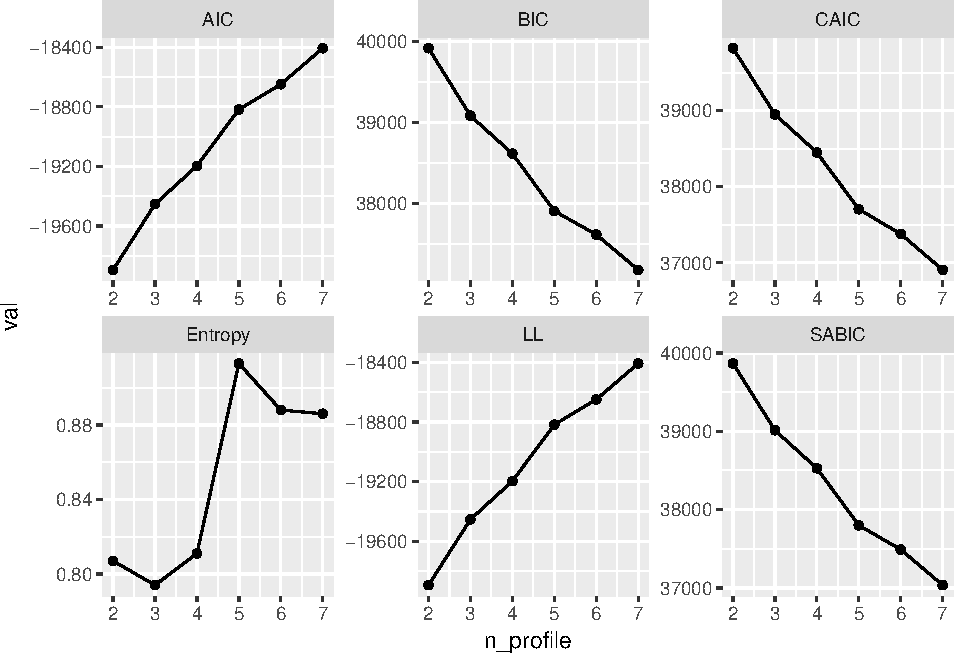
\includegraphics{rosenberg-dissertation_files/figure-latex/compare-solutions-model1-1.pdf}

\section{2. Just for model 2}\label{just-for-model-2}

\begin{Shaded}
\begin{Highlighting}[]
\NormalTok{d <-}\StringTok{ }\KeywordTok{compare_solutions_mplus}\NormalTok{(df,  }
\NormalTok{                             dm_cog_eng, dm_beh_eng, dm_aff_eng, dm_challenge, dm_competence,}
                             \DataTypeTok{starts =} \KeywordTok{c}\NormalTok{(}\DecValTok{600}\NormalTok{, }\DecValTok{120}\NormalTok{),}
                             \DataTypeTok{model =} \KeywordTok{c}\NormalTok{(}\DecValTok{2}\NormalTok{),}
                             \DataTypeTok{n_profiles_min =} \DecValTok{2}\NormalTok{, }
                             \DataTypeTok{n_profiles_max =} \DecValTok{10}\NormalTok{,}
                             \DataTypeTok{return_stats_df =} \OtherTok{TRUE}\NormalTok{,}
                             \DataTypeTok{include_BLRT=}\OtherTok{TRUE}\NormalTok{,}
                             \DataTypeTok{n_processors =} \DecValTok{8}\NormalTok{)}
\end{Highlighting}
\end{Shaded}

\begin{verbatim}
##   n_profiles model_2                         V3
## 1          2      NA                  38423.266
## 2          3      NA                  38049.877
## 3          4      NA                  37623.057
## 4          5      NA                  37301.328
## 5          6      NA Warning: LL not replicated
## 6          7      NA                   34517.58
## 7          8      NA Warning: LL not replicated
## 8          9      NA Warning: LL not replicated
## 9         10      NA Warning: LL not replicated
\end{verbatim}

\begin{Shaded}
\begin{Highlighting}[]
\NormalTok{d}
\end{Highlighting}
\end{Shaded}

\begin{verbatim}
##   n_profile model        LL       AIC      BIC    SABIC     CAIC Entropy
## 1         2     2 -19107.73 -19107.73 38423.27 38340.65 38267.95   0.924
## 2         3     2 -18897.06 -18897.06 38049.88 37948.20 37858.85   0.880
## 3         4     2 -18659.68 -18659.68 37623.06 37502.32 37396.37   0.922
## 4         5     2 -18474.83 -18474.83 37301.33 37161.52 37039.03   0.901
## 5         7     2 -17035.01 -17035.01 34517.58 34339.65 34184.21   0.965
##   VLMR_val VLMR_p   LMR_val  LMR_p BLRT_val BLRT_p
## 1  850.304      0   832.934 0.0000  850.304      0
## 2  421.343      0   412.736 0.0000  421.343      0
## 3  474.773      0   465.075 0.0000  474.773      0
## 4  304.938      0   298.709 0.0000  304.938      0
## 5       NA     NA -1374.094 0.8708       NA     NA
\end{verbatim}

\begin{Shaded}
\begin{Highlighting}[]
\NormalTok{d }\OperatorTok\StringTok{ }
\StringTok{    }\KeywordTok{select}\NormalTok{(n_profile}\OperatorTok{:}\NormalTok{CAIC, Entropy) }\OperatorTok\StringTok{ }
\StringTok{    }\KeywordTok{gather}\NormalTok{(key, val, }\OperatorTok{-}\NormalTok{n_profile, }\OperatorTok{-}\NormalTok{model) }\OperatorTok\StringTok{ }
\StringTok{    }\KeywordTok{ggplot}\NormalTok{(}\KeywordTok{aes}\NormalTok{(}\DataTypeTok{x =}\NormalTok{ n_profile, }\DataTypeTok{y =}\NormalTok{ val)) }\OperatorTok{+}
\StringTok{    }\KeywordTok{geom_point}\NormalTok{() }\OperatorTok{+}
\StringTok{    }\KeywordTok{geom_line}\NormalTok{() }\OperatorTok{+}
\StringTok{    }\KeywordTok{facet_wrap}\NormalTok{(}\StringTok{"key"}\NormalTok{, }\DataTypeTok{scales =} \StringTok{"free"}\NormalTok{)}
\end{Highlighting}
\end{Shaded}

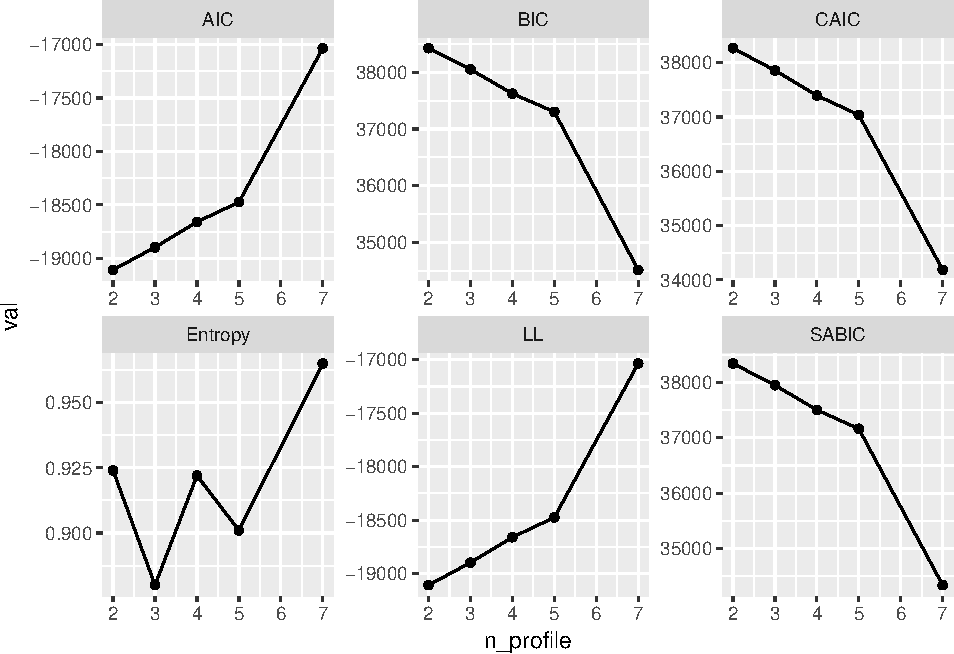
\includegraphics{rosenberg-dissertation_files/figure-latex/compare-solutions-model2-1.pdf}

\section{4. Some specific solutions for model
1}\label{some-specific-solutions-for-model-1}

\begin{Shaded}
\begin{Highlighting}[]
\NormalTok{m1_}\DecValTok{3}\NormalTok{ <-}\StringTok{ }\KeywordTok{estimate_profiles_mplus}\NormalTok{(df,  }
\NormalTok{                             dm_cog_eng, dm_beh_eng, dm_aff_eng, dm_challenge, dm_competence,}
                             \DataTypeTok{starts =} \KeywordTok{c}\NormalTok{(}\DecValTok{600}\NormalTok{, }\DecValTok{120}\NormalTok{),}
                             \DataTypeTok{model =} \DecValTok{1}\NormalTok{,}
                             \DataTypeTok{n_profiles =} \DecValTok{3}\NormalTok{,}
                             \DataTypeTok{include_BLRT=}\OtherTok{TRUE}\NormalTok{,}
                             \DataTypeTok{n_processors =} \DecValTok{8}\NormalTok{, }\DataTypeTok{remove_tmp_files =} \OtherTok{FALSE}\NormalTok{)}

\KeywordTok{plot_profiles_mplus}\NormalTok{(m1_}\DecValTok{3}\NormalTok{)}
\end{Highlighting}
\end{Shaded}

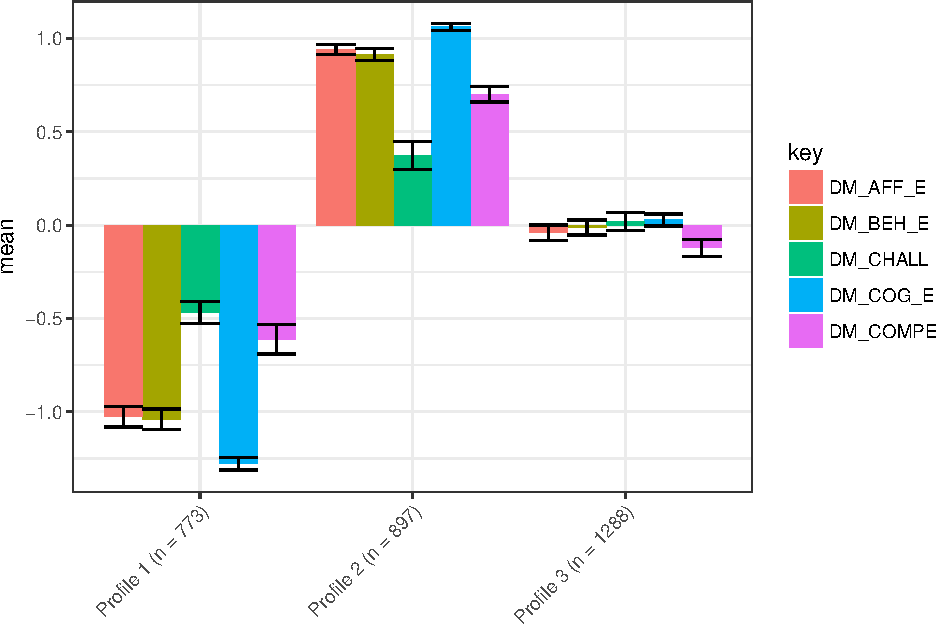
\includegraphics{rosenberg-dissertation_files/figure-latex/spec-solutions-model1-1.pdf}

\begin{Shaded}
\begin{Highlighting}[]
\KeywordTok{extract_LL_mplus}\NormalTok{()}
\end{Highlighting}
\end{Shaded}

\begin{verbatim}
## # A tibble: 119 x 3
##    LL           seed m_iterations
##  * <fct>       <dbl> <chr>       
##  1 -19453.381 231281 542         
##  2 -19453.381 879211 453         
##  3 -19453.381 897782 545         
##  4 -19453.381 155622 507         
##  5 -19453.381 192071 142         
##  6 -19453.381 507154 387         
##  7 -19453.381 674171 195         
##  8 -19453.381 316165 299         
##  9 -19453.381 374219 353         
## 10 -19453.381 783102 433         
## # ... with 109 more rows
\end{verbatim}

\begin{Shaded}
\begin{Highlighting}[]
\NormalTok{m1_}\DecValTok{4}\NormalTok{ <-}\StringTok{ }\KeywordTok{estimate_profiles_mplus}\NormalTok{(df,  }
\NormalTok{                             dm_cog_eng, dm_beh_eng, dm_aff_eng, dm_challenge, dm_competence,}
                             \DataTypeTok{starts =} \KeywordTok{c}\NormalTok{(}\DecValTok{600}\NormalTok{, }\DecValTok{120}\NormalTok{),}
                             \DataTypeTok{model =} \DecValTok{1}\NormalTok{,}
                             \DataTypeTok{n_profiles =} \DecValTok{4}\NormalTok{,}
                             \DataTypeTok{include_BLRT=}\OtherTok{TRUE}\NormalTok{,}
                             \DataTypeTok{n_processors =} \DecValTok{8}\NormalTok{, }\DataTypeTok{remove_tmp_files =} \OtherTok{FALSE}\NormalTok{)}

\KeywordTok{plot_profiles_mplus}\NormalTok{(m1_}\DecValTok{4}\NormalTok{)}
\end{Highlighting}
\end{Shaded}

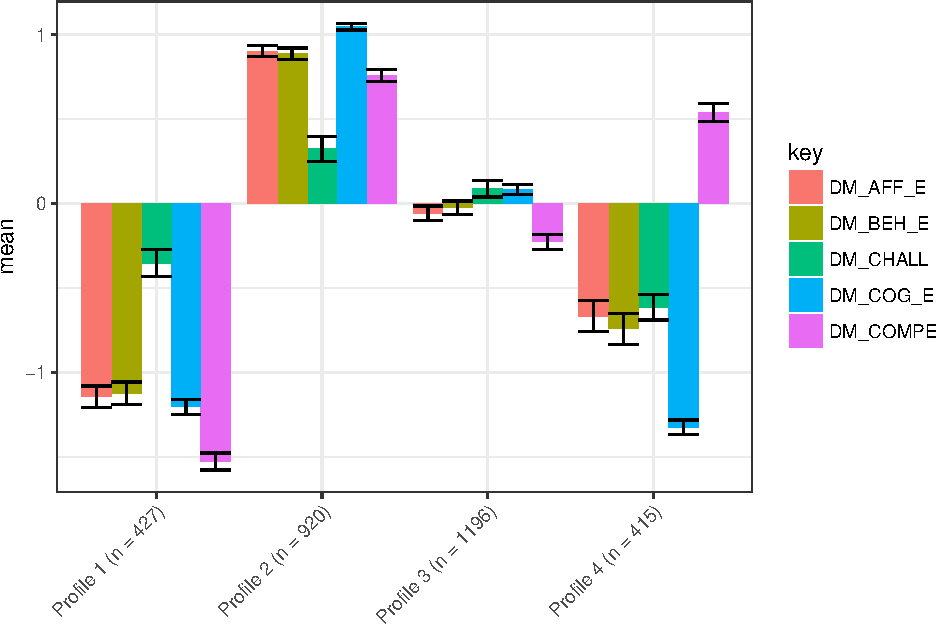
\includegraphics{rosenberg-dissertation_files/figure-latex/spec-solutions-model1-2.pdf}

\begin{Shaded}
\begin{Highlighting}[]
\KeywordTok{extract_LL_mplus}\NormalTok{()}
\end{Highlighting}
\end{Shaded}

\begin{verbatim}
## # A tibble: 80 x 3
##    LL           seed m_iterations
##  * <chr>       <dbl> <chr>       
##  1 -19196.328 415931 10          
##  2 -19196.328 260953 589         
##  3 -19196.328 576220 115         
##  4 -19196.328 329127 185         
##  5 -19196.328 391179 78          
##  6 -19196.328 352277 42          
##  7 -19196.328 443442 380         
##  8 -19196.328 518828 432         
##  9 -19196.328  36714 201         
## 10 -19196.328 456213 160         
## # ... with 70 more rows
\end{verbatim}

\begin{Shaded}
\begin{Highlighting}[]
\NormalTok{m1_}\DecValTok{5}\NormalTok{ <-}\StringTok{ }\KeywordTok{estimate_profiles_mplus}\NormalTok{(df,  }
\NormalTok{                             dm_cog_eng, dm_beh_eng, dm_aff_eng, dm_challenge, dm_competence,}
                             \DataTypeTok{starts =} \KeywordTok{c}\NormalTok{(}\DecValTok{600}\NormalTok{, }\DecValTok{120}\NormalTok{),}
                             \DataTypeTok{model =} \DecValTok{1}\NormalTok{,}
                             \DataTypeTok{n_profiles =} \DecValTok{5}\NormalTok{,}
                             \DataTypeTok{include_BLRT=}\OtherTok{TRUE}\NormalTok{,}
                             \DataTypeTok{n_processors =} \DecValTok{8}\NormalTok{, }\DataTypeTok{remove_tmp_files =} \OtherTok{FALSE}\NormalTok{)}

\KeywordTok{plot_profiles_mplus}\NormalTok{(m1_}\DecValTok{5}\NormalTok{)}
\end{Highlighting}
\end{Shaded}

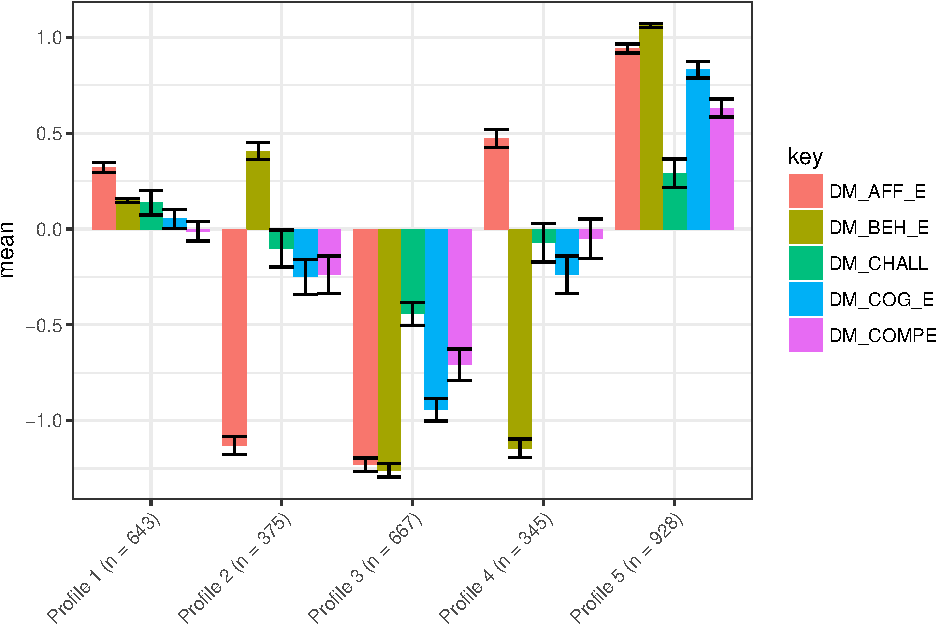
\includegraphics{rosenberg-dissertation_files/figure-latex/spec-solutions-model1-3.pdf}

\begin{Shaded}
\begin{Highlighting}[]
\KeywordTok{extract_LL_mplus}\NormalTok{()}
\end{Highlighting}
\end{Shaded}

\begin{verbatim}
## # A tibble: 82 x 3
##    LL           seed m_iterations
##  * <chr>       <dbl> <chr>       
##  1 -18817.934 152496 123         
##  2 -18817.934 602797 336         
##  3 -18817.934 432148 30          
##  4 -18817.934 399848 220         
##  5 -18837.053 387701 275         
##  6 -18858.428 850545 357         
##  7 -18858.428 298275 418         
##  8 -18858.428 626891 32          
##  9 -18944.968 823392 479         
## 10 -18944.968 147440 514         
## # ... with 72 more rows
\end{verbatim}

\begin{Shaded}
\begin{Highlighting}[]
\NormalTok{m1_}\DecValTok{6}\NormalTok{ <-}\StringTok{ }\KeywordTok{estimate_profiles_mplus}\NormalTok{(df,  }
\NormalTok{                             dm_cog_eng, dm_beh_eng, dm_aff_eng, dm_challenge, dm_competence,}
                             \DataTypeTok{starts =} \KeywordTok{c}\NormalTok{(}\DecValTok{600}\NormalTok{, }\DecValTok{120}\NormalTok{),}
                             \DataTypeTok{model =} \DecValTok{1}\NormalTok{,}
                             \DataTypeTok{n_profiles =} \DecValTok{6}\NormalTok{,}
                             \DataTypeTok{include_BLRT=}\OtherTok{TRUE}\NormalTok{,}
                             \DataTypeTok{n_processors =} \DecValTok{8}\NormalTok{, }\DataTypeTok{remove_tmp_files =} \OtherTok{FALSE}\NormalTok{)}

\KeywordTok{plot_profiles_mplus}\NormalTok{(m1_}\DecValTok{6}\NormalTok{)}
\end{Highlighting}
\end{Shaded}

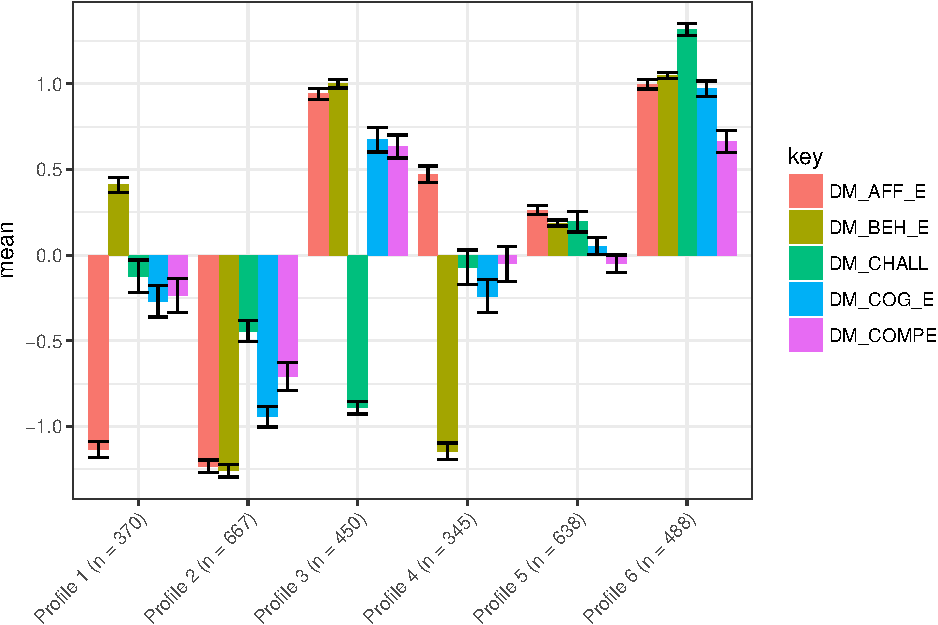
\includegraphics{rosenberg-dissertation_files/figure-latex/spec-solutions-model1-4.pdf}

\begin{Shaded}
\begin{Highlighting}[]
\KeywordTok{extract_LL_mplus}\NormalTok{()}
\end{Highlighting}
\end{Shaded}

\begin{verbatim}
## # A tibble: 64 x 3
##    LL           seed m_iterations
##  * <chr>       <dbl> <chr>       
##  1 -18648.785   1548 384         
##  2 -18648.785 282464 283         
##  3 -18668.802 529496 343         
##  4 -18695.729  49221 254         
##  5 -18695.729 153394 429         
##  6 -18695.729 741888 138         
##  7 -18695.729  85114 385         
##  8 -18695.729 173191 422         
##  9 -18695.729 436460 89          
## 10 -18695.729 153942 31          
## # ... with 54 more rows
\end{verbatim}

\begin{Shaded}
\begin{Highlighting}[]
\NormalTok{m1_}\DecValTok{7}\NormalTok{ <-}\StringTok{ }\KeywordTok{estimate_profiles_mplus}\NormalTok{(df,  }
\NormalTok{                             dm_cog_eng, dm_beh_eng, dm_aff_eng, dm_challenge, dm_competence,}
                             \DataTypeTok{starts =} \KeywordTok{c}\NormalTok{(}\DecValTok{600}\NormalTok{, }\DecValTok{120}\NormalTok{),}
                             \DataTypeTok{model =} \DecValTok{1}\NormalTok{,}
                             \DataTypeTok{n_profiles =} \DecValTok{7}\NormalTok{,}
                             \DataTypeTok{include_BLRT=}\OtherTok{TRUE}\NormalTok{,}
                             \DataTypeTok{n_processors =} \DecValTok{8}\NormalTok{, }\DataTypeTok{remove_tmp_files =} \OtherTok{FALSE}\NormalTok{)}

\KeywordTok{plot_profiles_mplus}\NormalTok{(m1_}\DecValTok{7}\NormalTok{)}
\end{Highlighting}
\end{Shaded}

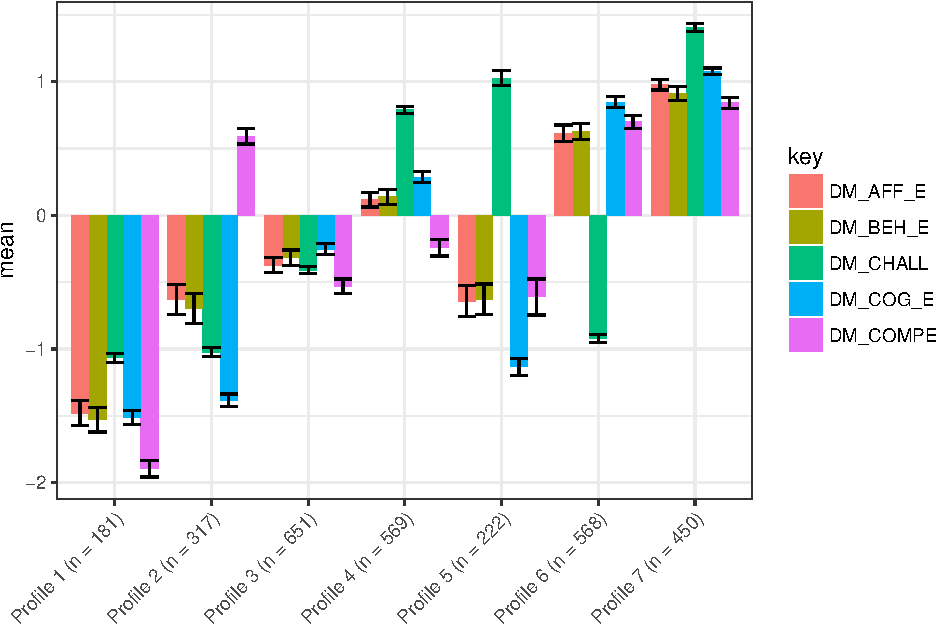
\includegraphics{rosenberg-dissertation_files/figure-latex/spec-solutions-model1-5.pdf}

\begin{Shaded}
\begin{Highlighting}[]
\KeywordTok{extract_LL_mplus}\NormalTok{()}
\end{Highlighting}
\end{Shaded}

\begin{verbatim}
## # A tibble: 52 x 3
##    LL           seed m_iterations
##  * <chr>       <dbl> <chr>       
##  1 -18407.232 475420 71          
##  2 -18407.232 871438 561         
##  3 -18469.834 597614 284         
##  4 -18469.834 830570 369         
##  5 -18469.834 283492 435         
##  6 -18469.834 260953 589         
##  7 -18518.118 153394 429         
##  8 -18634.678 950604 172         
##  9 -18660.958 922596 456         
## 10 -18662.856 160326 546         
## # ... with 42 more rows
\end{verbatim}

\begin{Shaded}
\begin{Highlighting}[]
\NormalTok{m1_}\DecValTok{7}\NormalTok{ <-}\StringTok{ }\KeywordTok{estimate_profiles_mplus}\NormalTok{(df,  }
\NormalTok{                             dm_cog_eng, dm_beh_eng, dm_aff_eng, dm_challenge, dm_competence,}
                             \DataTypeTok{starts =} \KeywordTok{c}\NormalTok{(}\DecValTok{600}\NormalTok{, }\DecValTok{120}\NormalTok{),}
                             \DataTypeTok{model =} \DecValTok{1}\NormalTok{,}
                             \DataTypeTok{n_profiles =} \DecValTok{7}\NormalTok{,}
                             \DataTypeTok{include_BLRT=}\OtherTok{TRUE}\NormalTok{,}
                             \DataTypeTok{n_processors =} \DecValTok{8}\NormalTok{, }\DataTypeTok{remove_tmp_files =} \OtherTok{FALSE}\NormalTok{, }\DataTypeTok{optseed =} \DecValTok{597614}\NormalTok{)}

\KeywordTok{plot_profiles_mplus}\NormalTok{(m1_}\DecValTok{7}\NormalTok{)}
\end{Highlighting}
\end{Shaded}

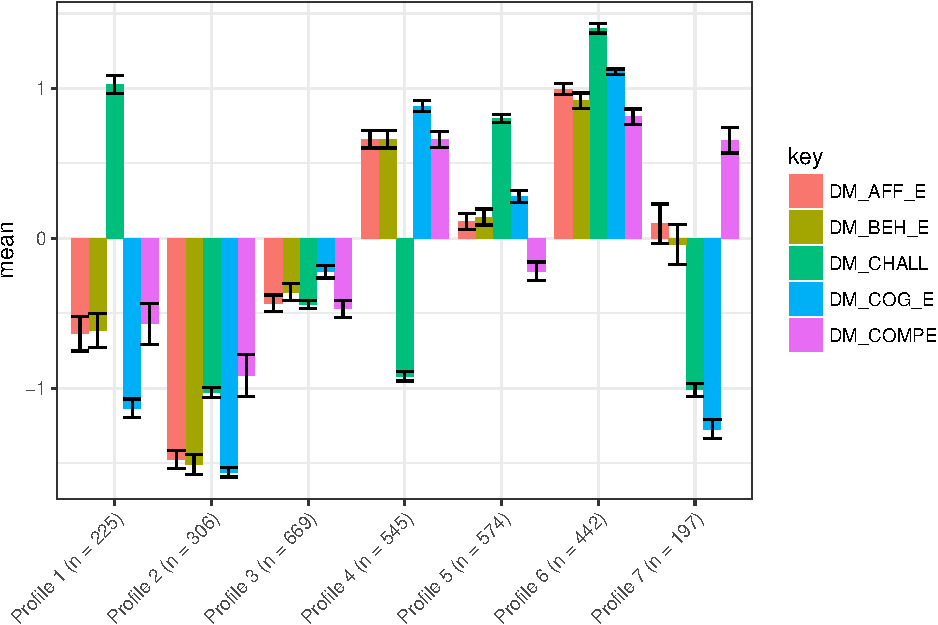
\includegraphics{rosenberg-dissertation_files/figure-latex/anotherm1-7-solution-1.pdf}

\begin{Shaded}
\begin{Highlighting}[]
\CommentTok{# extract_LL_mplus()}
\end{Highlighting}
\end{Shaded}

\section{5. Some specific solutions for model
2}\label{some-specific-solutions-for-model-2}

\begin{Shaded}
\begin{Highlighting}[]
\NormalTok{m1_}\DecValTok{3}\NormalTok{ <-}\StringTok{ }\KeywordTok{estimate_profiles_mplus}\NormalTok{(df,  }
\NormalTok{                             dm_cog_eng, dm_beh_eng, dm_aff_eng, dm_challenge, dm_competence,}
                             \DataTypeTok{starts =} \KeywordTok{c}\NormalTok{(}\DecValTok{600}\NormalTok{, }\DecValTok{120}\NormalTok{),}
                             \DataTypeTok{model =} \DecValTok{2}\NormalTok{,}
                             \DataTypeTok{n_profiles =} \DecValTok{3}\NormalTok{,}
                             \DataTypeTok{include_BLRT=}\OtherTok{TRUE}\NormalTok{,}
                             \DataTypeTok{n_processors =} \DecValTok{8}\NormalTok{, }\DataTypeTok{remove_tmp_files =} \OtherTok{FALSE}\NormalTok{)}

\KeywordTok{plot_profiles_mplus}\NormalTok{(m1_}\DecValTok{3}\NormalTok{)}
\end{Highlighting}
\end{Shaded}

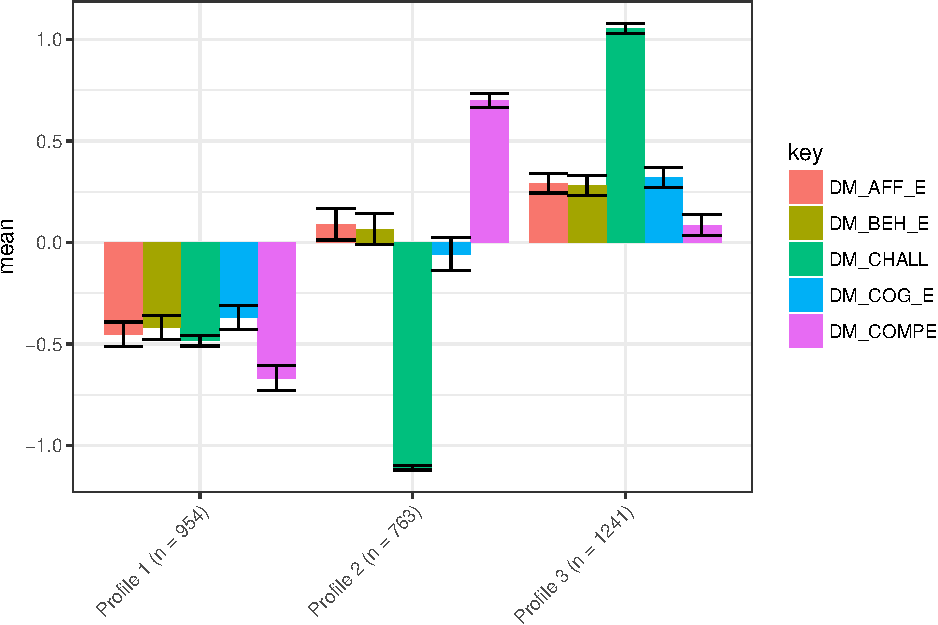
\includegraphics{rosenberg-dissertation_files/figure-latex/spec-solutions-model2-3-1.pdf}

\begin{Shaded}
\begin{Highlighting}[]
\KeywordTok{extract_LL_mplus}\NormalTok{()}
\end{Highlighting}
\end{Shaded}

\begin{verbatim}
## # A tibble: 120 x 3
##    LL           seed m_iterations
##  * <chr>       <dbl> <chr>       
##  1 -18897.062 154575 539         
##  2 -18897.062 606576 151         
##  3 -18897.062 746978 410         
##  4 -18897.062 107446 12          
##  5 -18897.062  30098 209         
##  6 -18897.062 871851 257         
##  7 -18897.062 491970 563         
##  8 -18897.062  76451 211         
##  9 -18897.062 152496 123         
## 10 -18897.062 458181 189         
## # ... with 110 more rows
\end{verbatim}

\begin{Shaded}
\begin{Highlighting}[]
\NormalTok{m1_}\DecValTok{4}\NormalTok{ <-}\StringTok{ }\KeywordTok{estimate_profiles_mplus}\NormalTok{(df,  }
\NormalTok{                             dm_cog_eng, dm_beh_eng, dm_aff_eng, dm_challenge, dm_competence,}
                             \DataTypeTok{starts =} \KeywordTok{c}\NormalTok{(}\DecValTok{600}\NormalTok{, }\DecValTok{120}\NormalTok{),}
                             \DataTypeTok{model =} \DecValTok{2}\NormalTok{,}
                             \DataTypeTok{n_profiles =} \DecValTok{4}\NormalTok{,}
                             \DataTypeTok{include_BLRT=}\OtherTok{TRUE}\NormalTok{,}
                             \DataTypeTok{n_processors =} \DecValTok{8}\NormalTok{, }\DataTypeTok{remove_tmp_files =} \OtherTok{FALSE}\NormalTok{)}

\KeywordTok{plot_profiles_mplus}\NormalTok{(m1_}\DecValTok{4}\NormalTok{)}
\end{Highlighting}
\end{Shaded}

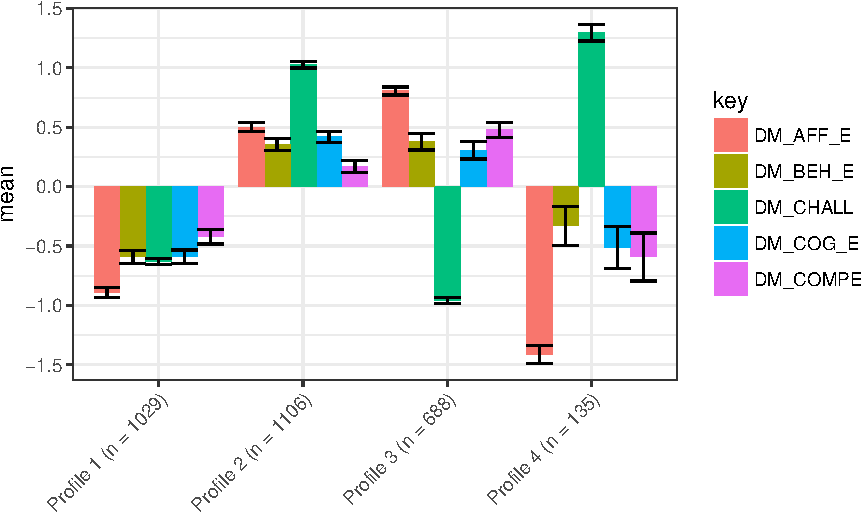
\includegraphics{rosenberg-dissertation_files/figure-latex/spec-solutions-model2-4-1.pdf}

\begin{Shaded}
\begin{Highlighting}[]
\KeywordTok{extract_LL_mplus}\NormalTok{()}
\end{Highlighting}
\end{Shaded}

\begin{verbatim}
## # A tibble: 119 x 3
##    LL           seed m_iterations
##  * <chr>       <dbl> <chr>       
##  1 -18659.676 286735 175         
##  2 -18659.676 349562 359         
##  3 -18659.676 568859 49          
##  4 -18686.131 562716 300         
##  5 -18690.761 475420 71          
##  6 -18690.761 147440 514         
##  7 -18690.761 279850 555         
##  8 -18690.761 667250 318         
##  9 -18690.761 153394 429         
## 10 -18709.289 327475 518         
## # ... with 109 more rows
\end{verbatim}

\begin{Shaded}
\begin{Highlighting}[]
\NormalTok{m1_}\DecValTok{5}\NormalTok{ <-}\StringTok{ }\KeywordTok{estimate_profiles_mplus}\NormalTok{(df,  }
\NormalTok{                             dm_cog_eng, dm_beh_eng, dm_aff_eng, dm_challenge, dm_competence,}
                             \DataTypeTok{starts =} \KeywordTok{c}\NormalTok{(}\DecValTok{600}\NormalTok{, }\DecValTok{120}\NormalTok{),}
                             \DataTypeTok{model =} \DecValTok{2}\NormalTok{,}
                             \DataTypeTok{n_profiles =} \DecValTok{5}\NormalTok{,}
                             \DataTypeTok{include_BLRT=}\OtherTok{TRUE}\NormalTok{,}
                             \DataTypeTok{n_processors =} \DecValTok{8}\NormalTok{, }\DataTypeTok{remove_tmp_files =} \OtherTok{FALSE}\NormalTok{)}

\KeywordTok{plot_profiles_mplus}\NormalTok{(m1_}\DecValTok{5}\NormalTok{)}
\end{Highlighting}
\end{Shaded}

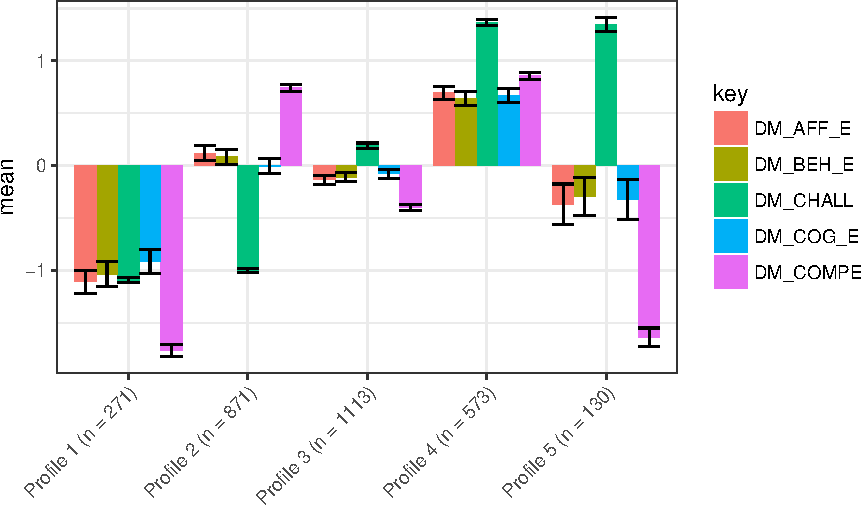
\includegraphics{rosenberg-dissertation_files/figure-latex/spec-solutions-model2-5-1.pdf}

\begin{Shaded}
\begin{Highlighting}[]
\KeywordTok{extract_LL_mplus}\NormalTok{()}
\end{Highlighting}
\end{Shaded}

\begin{verbatim}
## # A tibble: 114 x 3
##    LL           seed m_iterations
##  * <chr>       <dbl> <chr>       
##  1 -18474.834 154575 539         
##  2 -18474.834 436460 89          
##  3 -18474.834 746978 410         
##  4 -18474.834  85114 385         
##  5 -18479.167 217130 443         
##  6 -18479.167 539389 544         
##  7 -18481.815 407108 366         
##  8 -18481.815 165853 105         
##  9 -18481.815  73576 213         
## 10 -18481.815 471398 74          
## # ... with 104 more rows
\end{verbatim}

\begin{Shaded}
\begin{Highlighting}[]
\NormalTok{m1_}\DecValTok{6}\NormalTok{ <-}\StringTok{ }\KeywordTok{estimate_profiles_mplus}\NormalTok{(df,  }
\NormalTok{                             dm_cog_eng, dm_beh_eng, dm_aff_eng, dm_challenge, dm_competence,}
                             \DataTypeTok{starts =} \KeywordTok{c}\NormalTok{(}\DecValTok{600}\NormalTok{, }\DecValTok{120}\NormalTok{),}
                             \DataTypeTok{model =} \DecValTok{2}\NormalTok{,}
                             \DataTypeTok{n_profiles =} \DecValTok{6}\NormalTok{,}
                             \DataTypeTok{include_BLRT=}\OtherTok{TRUE}\NormalTok{,}
                             \DataTypeTok{n_processors =} \DecValTok{8}\NormalTok{, }\DataTypeTok{remove_tmp_files =} \OtherTok{FALSE}\NormalTok{)}

\KeywordTok{extract_LL_mplus}\NormalTok{()}
\end{Highlighting}
\end{Shaded}

\begin{verbatim}
## # A tibble: 104 x 3
##    LL           seed m_iterations
##  * <chr>       <dbl> <chr>       
##  1 -17098.434 344422 296         
##  2 -17216.914 226322 478         
##  3 -17714.856 853195 431         
##  4 -18285.363 153053 378         
##  5 -18304.150 211281 292         
##  6 -18304.150 529496 343         
##  7 -18320.492 350608 334         
##  8 -18323.206 691234 250         
##  9 -18337.703 425929 508         
## 10 -18337.703 153394 429         
## # ... with 94 more rows
\end{verbatim}

\begin{Shaded}
\begin{Highlighting}[]
\NormalTok{m1_}\DecValTok{7}\NormalTok{ <-}\StringTok{ }\KeywordTok{estimate_profiles_mplus}\NormalTok{(df,  }
\NormalTok{                             dm_cog_eng, dm_beh_eng, dm_aff_eng, dm_challenge, dm_competence,}
                             \DataTypeTok{starts =} \KeywordTok{c}\NormalTok{(}\DecValTok{600}\NormalTok{, }\DecValTok{120}\NormalTok{),}
                             \DataTypeTok{model =} \DecValTok{2}\NormalTok{,}
                             \DataTypeTok{n_profiles =} \DecValTok{7}\NormalTok{,}
                             \DataTypeTok{include_BLRT=}\OtherTok{TRUE}\NormalTok{,}
                             \DataTypeTok{n_processors =} \DecValTok{8}\NormalTok{, }\DataTypeTok{remove_tmp_files =} \OtherTok{FALSE}\NormalTok{)}

\KeywordTok{plot_profiles_mplus}\NormalTok{(m1_}\DecValTok{7}\NormalTok{)}
\end{Highlighting}
\end{Shaded}

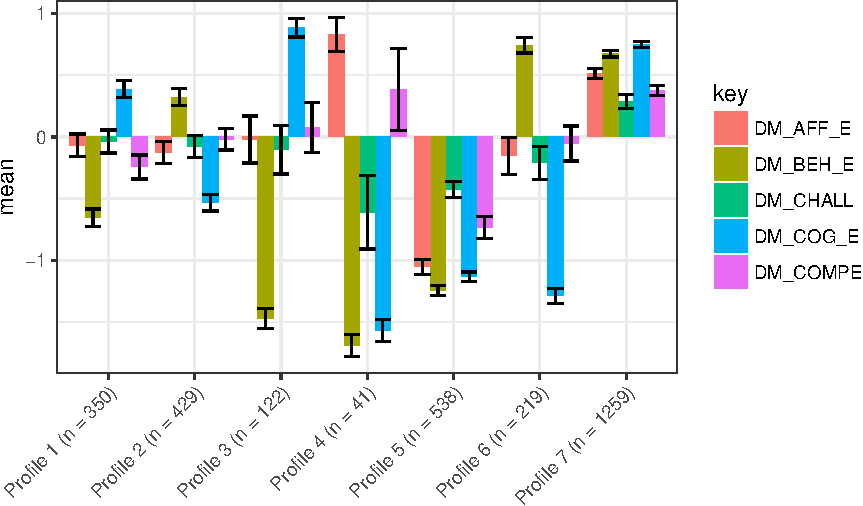
\includegraphics{rosenberg-dissertation_files/figure-latex/spec-solutions-model2-7-1.pdf}

\begin{Shaded}
\begin{Highlighting}[]
\KeywordTok{extract_LL_mplus}\NormalTok{()}
\end{Highlighting}
\end{Shaded}

\begin{verbatim}
## # A tibble: 97 x 3
##    LL           seed m_iterations
##  * <chr>       <dbl> <chr>       
##  1 -17035.006  85734 411         
##  2 -17035.006 344422 296         
##  3 -18213.406 939021 8           
##  4 -18214.792 458181 189         
##  5 -18217.063 715255 523         
##  6 -18227.574 126371 526         
##  7 -18227.574 391949 295         
##  8 -18234.603  30098 209         
##  9 -18234.603 150531 154         
## 10 -18234.603 790452 303         
## # ... with 87 more rows
\end{verbatim}

\chapter{Discussion}\label{discussion}

\chapter{Discussion}\label{discussion-1}

Placeholder

\chapter{Appendix}\label{appendix}

\bibliography{book.bib,packages.bib}


\end{document}
